\documentclass[]{elsarticle} %review=doublespace preprint=single 5p=2 column
%%% Begin My package additions %%%%%%%%%%%%%%%%%%%
\usepackage[hyphens]{url}

  \journal{Global Environmental Change} % Sets Journal name


\usepackage{lineno} % add
  \linenumbers % turns line numbering on
\providecommand{\tightlist}{%
  \setlength{\itemsep}{0pt}\setlength{\parskip}{0pt}}

\usepackage{graphicx}
\usepackage{booktabs} % book-quality tables
%%%%%%%%%%%%%%%% end my additions to header

\usepackage[T1]{fontenc}
\usepackage{lmodern}
\usepackage{amssymb,amsmath}
\usepackage{ifxetex,ifluatex}
\usepackage{fixltx2e} % provides \textsubscript
% use upquote if available, for straight quotes in verbatim environments
\IfFileExists{upquote.sty}{\usepackage{upquote}}{}
\ifnum 0\ifxetex 1\fi\ifluatex 1\fi=0 % if pdftex
  \usepackage[utf8]{inputenc}
\else % if luatex or xelatex
  \usepackage{fontspec}
  \ifxetex
    \usepackage{xltxtra,xunicode}
  \fi
  \defaultfontfeatures{Mapping=tex-text,Scale=MatchLowercase}
  \newcommand{\euro}{€}
\fi
% use microtype if available
\IfFileExists{microtype.sty}{\usepackage{microtype}}{}
\bibliographystyle{elsarticle-harv}
\ifxetex
  \usepackage[setpagesize=false, % page size defined by xetex
              unicode=false, % unicode breaks when used with xetex
              xetex]{hyperref}
\else
  \usepackage[unicode=true]{hyperref}
\fi
\hypersetup{breaklinks=true,
            bookmarks=true,
            pdfauthor={},
            pdftitle={Mobility and flexibility enable resilience of human harvesters to environmental perturbation},
            colorlinks=false,
            urlcolor=blue,
            linkcolor=magenta,
            pdfborder={0 0 0}}
\urlstyle{same}  % don't use monospace font for urls

\setcounter{secnumdepth}{5}
% Pandoc toggle for numbering sections (defaults to be off)

% Pandoc citation processing

% Pandoc header



\begin{document}
\begin{frontmatter}

  \title{Mobility and flexibility enable resilience of human harvesters to
environmental perturbation}
      
  \begin{abstract}
  Characteristics of natural resources that enable sustainable management
  are often more fully understood than the adaptive behaviors of human
  harvesters in those same systems. Given increasing environmental
  variability due to climate change, it is especially critical to
  understand how human harvesters may respond to environmental
  perturbation. In this study, we identify characteristics that promoted
  resilience of one the most valuable fisheries on the west coast of the
  United States to a record marine heatwave. Using movement telemetry
  linked to fishery landings records from more than 500 fishing vessels,
  encompassing 2.2 million geolocations and more than \$2 billion in
  revenue, we found that vessels employed two, non-mutually exclusive
  strategies to cope with the anomalous environmental and management
  conditions imposed by the heatwave: increasing spatial mobility and
  diversifying fishery participation. The combination of these strategies
  appeared to be the most adaptive, as it produced the greatest increase
  in profits. In contrast, participants that specialized in a single
  fishery and concentrated fishing effort in small spatial areas
  experienced the greatest losses driven by the heatwave. Our data-driven
  approach reveals behaviors that can be promoted to improve the adaptive
  capacity of human harvesters in an era of unprecedented environmental
  perturbation.
  \end{abstract}
   \begin{keyword} climate change adaptation \textbar{} environmental perturbation
\textbar{} marine heatwave \textbar{} fisheries dynamics\end{keyword}
 \end{frontmatter}

\hypertarget{intro}{%
\section{Introduction}\label{intro}}

Sustainability in social-ecological systems---the continued provision of
human and ecological benefits from healthy ecosystems (Leslie et al.,
2015)---requires resilience to environmental perturbations. Often,
though, people respond to environmental change in diverse and complex
ways. Just as multiple species occupying similar ecological niches may
react differently to physical changes in their environments (Elmqvist et
al., 2003), human actors in a social-ecological system can exhibit
diverse behaviors within the constraints imposed by the governance
system (Mcginnis and Ostrom, 2014). Groups of resource users with
distinct livelihood portfolios, available capital, or spatial patterns
of resource extraction will not respond the same way to environmental or
management changes (Young et al., 2019). In response to change, some
users might stick to established knowledge and reliable spatial patterns
of exploitation, while others might employ more exploratory strategies
that carry higher potential upsides but also higher risks and costs
(Cohen et al., 2007). Understanding the adaptive behaviors of resource
users is all the more important given the increasing prevalence of
extreme climate events attributable to climate change (Abatzoglou et
al., 2019; Cook et al., 2018; Oliver et al., 2018; Townhill et al.,
2018), but empirical evidence making the link between climate extremes
and contemporaneous human adaptation remains lacking.

Fisheries are a prominent example of a social-ecological system where
complex links between resource user (harvester) behavior and natural
resource dynamics drive sustainability (Branch et al., 2006). Fisheries
represent the last large-scale wild harvest of food on Earth, but also
one of the most traditional livelihoods in human history. Difficulties
in achieving sustainability in fisheries have often been linked to an
inadequate understanding of harvester dynamics (Fulton et al., 2011;
Hilborn, 1985). Differences in fisher behaviors, both within and across
fisheries, can affect the stability and sustainability of fish
populations (Fryxell et al., 2017; Salas and Gaertner, 2004), of other
species---for instance, endangered marine mammals or seabirds---and of
the fishery itself (Gladics et al., 2017; Hamilton and Baker, 2019).

Additionally, different behavioral segments of fishing fleets may
respond in different ways to management measures, or may be
differentially vulnerable to environmental perturbations (Salas and
Gaertner, 2004). For example, O'Farrell, Sanchirico, et al. (2019) found
that more exploratory fishing vessels---those that, on average, traveled
further and more often traversed new fishing grounds---were better able
to cope with an extended spatial closure. Heterogeneous behavioral
responses of fishers can be difficult to study, despite their potential
impact on resource dynamics. Partly, this is due to a lack of detailed
spatial and economic information on harvester behavior. However, recent
years have seen a rise in availability of these types of fishery data,
paired with methods to extract behavioral insights from them (Joo et
al., 2015; Mendo et al., 2019; Watson and Haynie, 2016). In the
following, we apply a range of data-driven methods to ask: how did human
harvesters cope with and adapt to a major environmental perturbation in
the most valuable fishery on the U.S. west coast?

The Dungeness crab fishery on the west coast of the United States often
obtains in excess of \$200 million in revenue from over 1,000
participating vessels each year (Rasmuson, 2013; Richerson et al.,
2020). It is a fishery that is central both ecologically and
economically (Fuller et al., 2017) to the west coast social-ecological
system, making it at once a cornerstone of fishers' portfolios and a
source of complexity in fisheries governance (Holland and Leonard, 2020;
Holland et al., 2017). Dungeness crab populations appear able to
withstand immense fishing pressure, and although crab abundance can
fluctuate markedly from year to year, long term abundance has been
relatively stable for more than a half century (Richerson et al., 2020).
Harvester characteristics vary widely for an industrialized
fishery---Dungeness crab vessels have a large range of sizes (in our
data, 21 to 103 feet), and operate out of both large urban and small
rural fishing ports across the U.S. west coast.

Recent environmental shocks have challenged the social and economic
sustainability of the Dungeness crab fishery. In 2014-2016, a record
marine heatwave (MHW) led to a harmful algal bloom of unprecedented
scale (McCabe et al., 2016), causing toxin levels in Dungeness crabs to
reach levels dangerous for human consumption and correspondingly lengthy
delays in large regions of the coast in the 2015-16 and 2016-17
Dungeness fishing seasons. Concurrently, the MHW caused shoreward
compression of the preferred feeding habitat of large whales,
contributing to a rise in entanglements of whales in Dungeness crab
fishing gear and increasing risk of fishery closure due to marine mammal
interactions, effects that continued to directly affect fishery closures
through the 2017-18 Dungeness crab season (Feist et al., 2021; Santora
et al., 2020). During this period, Dungeness crab fishers had to contend
with significant ecological changes and the management measures those
changes precipitated. Like with climate extremes in other systems (Loon
et al., 2016), the effects of this MHW were complex, reverberated
through the social-ecological system, and persisted for years after the
anomalous warming dissipated (Fisher et al., 2021; Smale et al., 2019;
Suryan et al., 2021). While much recent literature is dedicated to
examination of biophysical and ecological impacts of the MHW (Cavole et
al., 2016; McCabe et al., 2016; von Biela et al., 2019), to date far
less attention has been given to exploring how social systems cope and
change with these perturbations (Fisher et al., 2021; Jardine et al.,
2020; K. M. Moore et al., 2020).

In this study, we compare the adaptive responses of behavioral groups
within the Dungeness crab fishery to the multi-year MHW that directly
affected the 2015-16 through 2017-18 Dungeness crab seasons. The 2015-16
Dungeness crab season was the first season to be significantly delayed
as a direct result of ecosystem changes, a trend that continued through
the 2017-18 season. While previous work has investigated economic
impacts (Holland and Leonard, 2020; Jardine et al., 2020; Mao and
Jardine, 2020) and changes in fishery participation due to the
MHW-associated harmful algal bloom (Fisher et al., 2021), here we
explicitly investigate and quantify fishers' adaptive spatial behaviors
in response to the MHW more broadly and for the full three-year period
over which the MHW impacts manifested. Using a 10-year time-series of
more than 2 million satellite-derived fishing vessel location records,
linked to fishery revenue and landings data, we derive quantitative
behavioral metrics describing space use and mobility of Dungeness crab
vessels, then organize these behaviors into characteristic behavioral
groups. We explore the overlap of spatial behaviors with profitability,
fishing season length, and revenue diversity. We track these behavioral
groups over time, and identify key behavioral metrics that promoted
adaptation during and after the MHW. This analysis therefore offers
insights into the types of adaptive behaviors that may promote
sustainable outcomes in other commercial fisheries and perhaps in
social-ecological systems more broadly.

\hypertarget{methods}{%
\section{Materials and Methods}\label{methods}}

\hypertarget{data-sources}{%
\subsection{Data sources}\label{data-sources}}

We used satellite-based Vessel Monitoring System (VMS) data and port
level fishery landings data to define most of the behavioral variables
used in the study. The VMS database is maintained by the National Marine
Fisheries Service's Office of Law Enforcement, and records the positions
of vessels at approximately one hour intervals. Similar VMS data has
been used in other studies of fishery spatial dynamics (Feist et al.,
2021; Joo et al., 2015; O'Farrell, Chollett, et al., 2019; Watson and
Haynie, 2016). A subset of the vessels that participate in the Dungeness
crab fishery are equipped with VMS transponders (primarily vessels that
also participate in the west coast groundfish fishery, where VMS
transponders are mandatory). This subset varies between 19 and 26
percent of all vessels recording landings for Dungeness crab between the
2008-2009 and 2018-2019 seasons, representing between 10 and 57 percent
of all Dungeness crab landings by weight, and between 15 and 42 percent
of Dungeness revenue, depending on the year and state (California,
Oregon, or Washington). Oregon has the highest relative VMS
representation, followed by California, then Washington.

Fish ticket information was obtained through the Pacific Fisheries
Information Network (PacFIN). These data represent 1949 vessels
targeting Dungeness crab in California, across more than 300,000 fish
tickets (i.e., fishing trips). Fishing trips were defined as targeting
Dungeness crab if the total landings of Dungeness on the individual fish
ticket were at least 10 percent greater than the landed weight of the
next greatest species.

We joined the fish ticket data to the VMS data through unique vessel
identification numbers and timestamps. VMS geolocations comprising a
fishing trip were defined as all of the geolocations between a landed
fish ticket and the one immediately preceding it (i.e., the previous
ticket landed by the same vessel). After joining the VMS and fish ticket
data, we removed the small number of trips in which the final VMS data
point for a trip was greater than 50km from the port of landing recorded
on the ticket, reasoning that these are unreliable records. Finally, we
removed VMS records from vessels sitting idle in port. To do so, we
truncated all but the first and last VMS records for each trip that fell
within a small buffer zone (1.5 to 3 km) around each port of landing and
with an average calculated speed of less than 0.75 m/s.

Dungeness crab fishing seasons on the west coast typically begin in the
middle of November (for Central California) or beginning of December
(for Northern California, Oregon, and Washington), but can be variable
in their starting dates, depending on state (California, Oregon, or
Washington), harmful algal bloom closures, price and market conditions,
crab condition and meat quality, and potential interactions with
protected species like humpback whales. Therefore, we used a data-driven
approach to define the start date for each crab season in each of the 20
fishing port groups on the west coast. Port groups are defined by PacFIN
and include clusters of small, neighboring fishing ports. For each port
group in each season, we found the date after October 31 of each season
that the total Dungeness crab landings into that port reached 1 percent
of the eventual, season-long landings. This approach identifies the
realized start date of the crab fishery in each portion of the coast in
each year.

The maximum length of a Dungeness fishing trip was defined as seven
days. That is, if there was a gap of greater than seven days between
consecutive tickets, the VMS geolocations greater than seven days prior
to the landed ticket were discarded. The final dataset comprises a clean
record of geolocations associated with each Dungeness crab fishing trip.

The only other data source used in the calculation of behavioral metrics
is a measure of average daily wind speeds, from AVHRR Pathfinder
satellite-derived measurements (https://data.nodc.noaa.gov;
https://doi.org/10.7289/v52j68xx). The data are modelled daily on a 0.04
degree grid (approximately 5 km at the equator) and are available from
1981-present.

\hypertarget{construction-of-fishing-behavioral-metrics}{%
\subsection{Construction of Fishing Behavioral
Metrics}\label{construction-of-fishing-behavioral-metrics}}

Fishing behavioral metrics were calculated from fish ticket, VMS, and
wind speed data. Our choice of behavioral variables to calculate was
driven by previous evidence of the importance of each variable in
describing fisher behavioral patterns (Fuller et al., 2017; Kasperski
and Holland, 2013; O'Farrell, Chollett, et al., 2019; O'Farrell,
Sanchirico, et al., 2019; Pfeiffer and Gratz, 2016). Each of the fisher
behavioral variables described one characteristic of a vessel's apparent
behavior over the course of a fishing season---a vessel-season. Cluster
analysis (see next section) was performed on these vessel-seasons, and
individual vessels could be clustered into different behavioral groups
in different seasons. To determine whether a vessel would be included in
the analysis, we calculated the total Dungeness crab revenue for each
vessel in each season from 2008-09 to 2018-19. The 5th percentile for
annual Dungeness revenue per vessel was \$5828. We retained all
vessel-seasons with greater than \$5828 in revenue in any season (i.e.,
we retain the top 95 percent of all vessel-seasons as measured by
revenue).

Our behavioral metrics fall into five general categories: port use,
fishing trip characteristics, participation in other fisheries,
risk-taking behavior, and exploration and mobility (see Table A.1 for
full technical definitions of metrics). Port use metrics include the
number of ports visited per fishing trip, ports visited per month,
diversity of port use (calculated as a Shannon diversity index on the
proportions of trips landed in each port), and the total number of ports
visited across the entire season. The trip metrics are the mean and
standard deviation of trip distance (in km) and duration (in days).
Vessel size has been used as a proxy for fleet segments in other studies
(Jardine et al., 2020). We did not include vessel size as a metric,
since vessel size alone is not a behavioral variable, but we explored
its relationship to included metrics as a point of comparison (Figs.
A.5, A.6).

Fishery participation metrics include season length, proportion of
revenue and fish tickets from other (non-Dungeness) fisheries, and
revenue diversity. The Dungeness fishery operates as a derby, where the
majority of the landings and profits are obtained in the first few
months of each season (Fig. A.4). Our season length metric captures this
phenomenon and indicates the day of the crab season that each vessel
reaches 90 percent of its cumulative landings for that season. To
calculate the proportion of revenue and tickets from other fisheries,
and revenue diversity, we use a version of the fish ticket data that
includes all fishery targets (not just Dungeness crab). Using these
tickets, the proportion of non-Dungeness revenue is calculated, as well
as the proportion of fish tickets submitted by that vessel with a target
other than Dungeness crab. Revenue diversity for each vessel-season is
an inverse Simpson index calculated on the proportion of revenue
obtained from each species in a vessel's fishing portfolio.

Risk-taking behavior is modelled after the definition in Pfeiffer and
Gratz (2016), who also studied west-coast fisheries, as propensity to
fish in high-wind conditions. Using the Pathfinder winds data, we
extracted the wind speed at each VMS location, then calculated the 95th
percentile of wind speed experienced by each vessel on each trip.
Finally, the risk-taking metric was defined as the proportion of trips
in a season where the 95th percentile of experienced wind speed was
greater than 7.5 m/s (Pfeiffer and Gratz, 2016).

Exploration and mobility were measured with home range and location
choice entropy, adopting the definitions in O'Farrell et al.~(2019).
Home range was calculated as the area of the minimum convex polygon
encompassing all VMS locations in a vessel-season, after removing the
five percent of locations that were the furthest from other points
(i.e., spatial outliers). Location choice entropy measures the
propensity of vessels to explore new locations versus returning to the
same locations, and is calculated cumulatively across each vessel's
fishing season (O'Farrell, Sanchirico, et al., 2019). Spatial locations
were defined as individual cells on a 5x5km grid. As a season
progresses, entropy increases as vessels explore novel locations and
decreases as the same locations are revisited repeatedly. The
season-long metric for exploration for each vessel is defined as the
90th percentile of maximum location choice entropy in that season.

Definitions of all metrics used in the clustering analysis are provided
in the Appendix.

\hypertarget{cluster-analysis}{%
\subsection{Cluster Analysis}\label{cluster-analysis}}

All metrics were checked for collinearity, and thinned such that no two
metrics had a Pearson correlation greater than 0.7. This thinning
removed mean and standard deviation of trip distance, total number of
visited ports, and proportion of non-Dungeness tickets from the
analysis. The remaining 11 metrics were scaled to range from zero to one
by dividing each metric by its maximum value (across all seasons).
Clustering was performed using Euclidean distances and Ward aggregation
that minimizes total within-cluster variance. The number of clusters was
determined using the Nbclust package in R (Charrad et al., 2014), which
calculates 22 clustering indices before recommending an optimal number
of clusters via majority vote amongst indices. Adopting the optimal
clusters defined by NbClust, we visualized results graphically using
principal component analysis. After vessel-seasons were assigned to
groups, we tested for differences between groups along specific
behavioral metrics using Tukey's HSD.

The importance of individual metrics in discriminating between clusters
was calculated using random forest analysis, utilizing the randomForest
package in R (Liaw and Wiener, 2002). Random forests were grown on
subsamples of the data to classify vessel-seasons according to their
defined clusters from the previous step. Then, these random forests were
used to predict withheld data. Variable importance was defined as the
increase in the rate of mis-classification of vessel-seasons into
clusters when the particular variable was randomly permuted.

\hypertarget{dungeness-fishing-profitability}{%
\subsection{Dungeness Fishing
Profitability}\label{dungeness-fishing-profitability}}

We used fish ticket data to assess the per-trip, per-week, and
per-season landings and revenue of vessels in each fisher behavioral
group over time. Additionally, we modeled fishing costs following the
approach of Dewees et al. (2004) to assign an estimated profit to each
fishing trip. The cost of a fishing trip \(C_t\) is assumed to be a
function of fuel \(C_f\) and bait costs, and the costs of labor (i.e.,
crew) \(C_c\):

\[C_t = C_f + C_c\] Fuel and bait cost is a function of vessel size
\(L\) and number of days fished \(d\), as well as trip year \(y\) to
adjust for an assumed 2 percent inflation rate.

\[C_f = f(L,d,y)\]

Crew cost is a function of vessel size (because larger vessels require
more crew members) and total trip revenue \(R\) (since crew members
receive a proportion of revenue).

\[C_c = f(L,R)\]

The above cost relationships were parameterized using data from Dewees
et al. (2004), who administered a survey to 243 Dungeness crab fishers
and compiled estimates of fishing costs by vessel size. The survey
estimated costs associated with bait, fuel, and labor (crew) for small
(less than 9.1m), medium (9.1-15.2 m) and large (greater than 15.2 m)
fishing vessels. Using the means and standard deviations of these costs
reported in Dewees et al. (2004), we simulated 10,000 trip costs for
vessels ranging in length from 6.4 to 31.4 m, which is the range of
vessel sizes in our data. Then, linear relationships between vessel size
and both types of costs were estimated with simple linear regression.
The resulting relationships,

\[C_f = d(150+3.5L)*1.02^{y-2004}\] \[C_c = R(0.17 + 0.0018L)\]

were used to deterministically assign a cost to each Dungeness fishing
trip in our data. From there, a profit for each trip could be estimated
by subtracting costs from revenue. Using trip-level profits, we
calculated mean profits per week---across seasons---for vessels in each
behavioral group, as well as season-long profits.

Using the fish ticket revenue data, we also calculated total revenue
from all non-Dungeness fisheries for each vessel-season in the analysis.
We constrained the calculation of non-Dungeness revenue to only those
fishing trips that occurred within each vessel's apparent Dungeness
season (that is, within the time period where the vessel was also
landing Dungeness crab).

\hypertarget{adaptation-to-the-marine-heatwave}{%
\subsection{Adaptation to the Marine
Heatwave}\label{adaptation-to-the-marine-heatwave}}

Using the results of cluster analyses, we compared key characteristics
of behavioral groups in MHW versus non-MHW crab seasons. We defined the
MHW as encompassing the crab fishing seasons from 2015-16 to 2017-18.
Although there is evidence that the MHW began affecting west coast
ecosystems as early as late 2014 (Cavole et al., 2016; McCabe et al.,
2016), the 2015-16 Dungeness crab season was the first to be
significantly delayed as a direct result of ecosystem changes (Jardine
et al., 2020), a trend that continued through the 2017-18 season.

Adopting this definition of the MHW period, we compared mean Dungeness
profit, non-Dungeness revenue (i.e., external fishery revenue), and home
range size over time among behavioral groups to assess potential
adaptive strategies. For each of these three comparisons, we performed a
two-way ANOVA to test for significant differences in mean profits,
revenue, and home range by behavioral group and period (non-MHW or MHW).

All analyses in the study were performed in R (R Core Team, 2021).

\hypertarget{results}{%
\section{Results}\label{results}}

\begin{figure}%[tbhp]
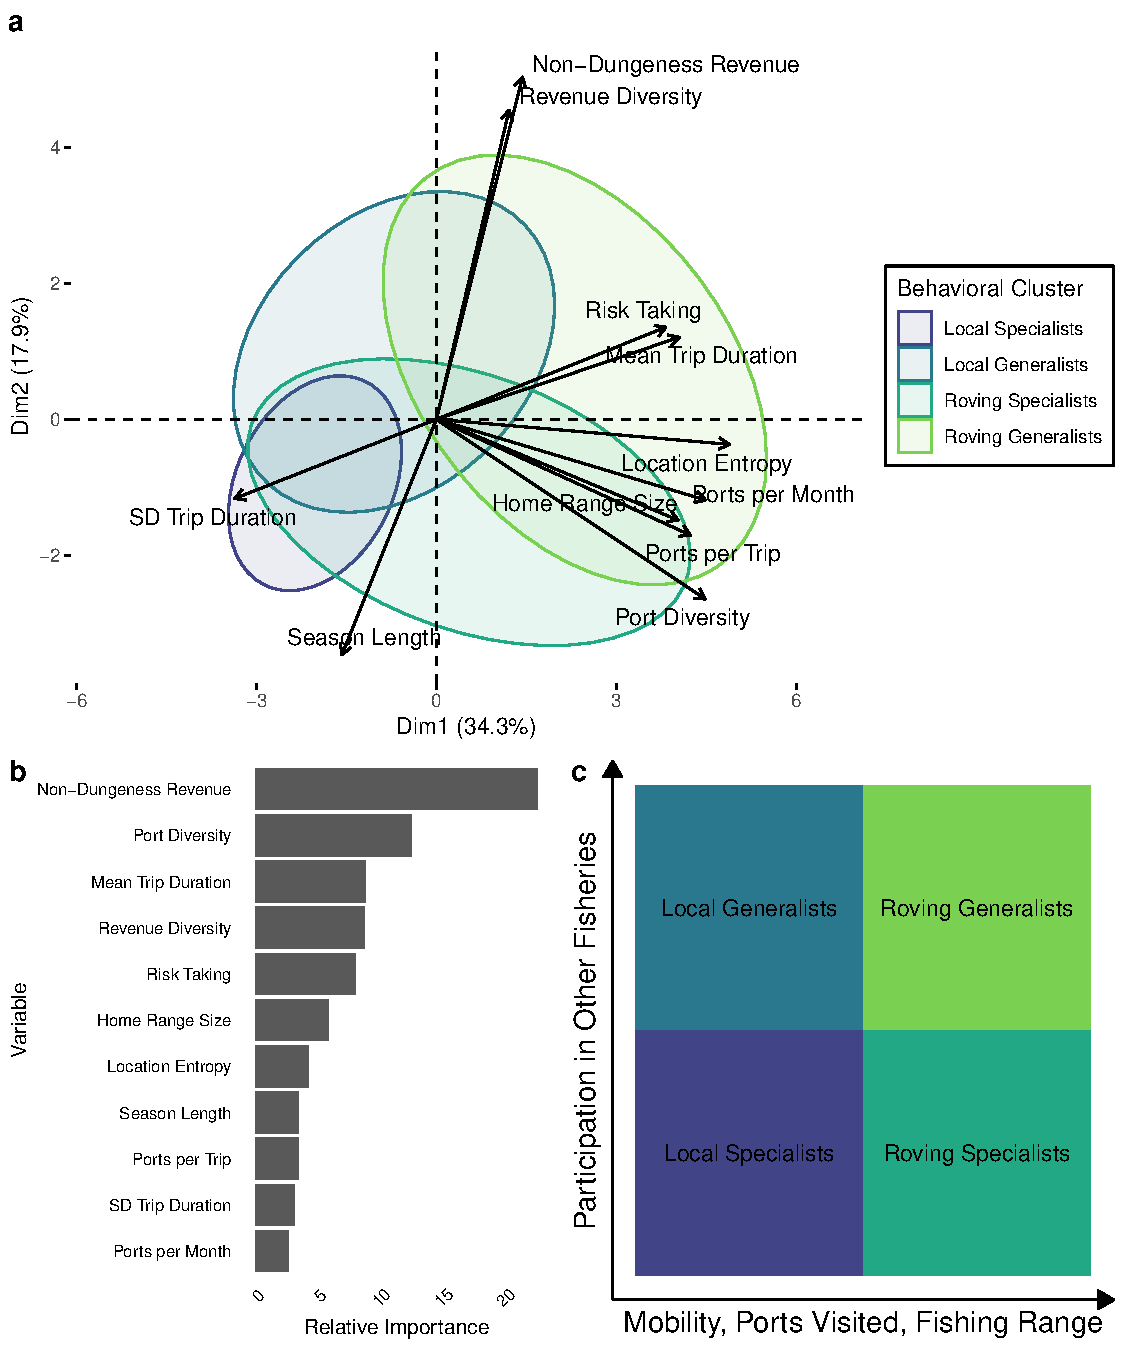
\includegraphics[width=\linewidth]{fig_pca_rf.pdf}
\caption{Data-driven formation of fishing behavioral groups. (a) Principal component analysis of vessel-seasons. Clusters of vessel-seasons, which determine behavioral groups, are enclosed by ellipses. Arrows represent the association between metrics in the cluster analysis relative to the placement of vessel-seasons. (b) Ranked importance of top variables used to classify vessel-seasons into behavioral groups, as determined by random forest analysis.(c) Conceptual visualization of the major axes defining behavioral groups.}
\label{fig:pca}
\end{figure}

\hypertarget{describing-fisher-behavior}{%
\subsection{Describing Fisher
Behavior}\label{describing-fisher-behavior}}

The combined vessel telemetry and fisheries landings dataset captured
the behaviors of 596 different vessels spanning 11 fishing seasons
(2008-2019), with \textasciitilde2.2 million satellite-derived Vessel
Monitoring System (VMS) geolocations, and 315,000 fishery landing
records. Using these combined data, we analyzed 11 behavioral variables
in five general behavioral categories: fishing port use, fishing trip
characteristics, participation in other fisheries, risk-taking behavior,
and exploration and mobility (definitions of all metrics are provided in
Table A.1).

The 3391 vessel-seasons in our data fell into four behavioral cluster
groups (Figs. \ref{fig:pca}a, A.1). The most important discriminating
variables driving the clustering according to random forest analysis
were proportion of revenue from non-Dungeness crab fisheries, followed
by diversity of port use, revenue diversity, and mean trip duration
(Fig. \ref{fig:pca}b). These analyses suggest that the behavior of the
four groups can be conceptualized as varying along two major axes (Fig.
\ref{fig:pca}c): (1) spatial mobility (principal component 1 in Fig.
\ref{fig:pca}a) and (2) propensity to fish in non-Dungeness crab
fisheries (fishery flexibility, principal component 2 in Fig.
\ref{fig:pca}a).

Vessels with higher spatial mobility, which we term Roving groups, move
between ports throughout a fishing season and have large fishing ranges,
while those with lower mobility---Local groups---show greater fidelity
to a single port. Vessels with greater fishery flexibility, deemed
Generalist groups, have high revenue diversity and derive a relatively
greater portion of their total fishery revenue from fisheries other than
Dungeness crab. Vessels exhibiting less
flexibility---Specialists---concentrate fishing effort within the
Dungeness crab fishery. A vessel-season is therefore defined as either
Roving or Local, and either Specialist or Generalist. As an example, for
crab vessels fishing out of Newport, Oregon, Local Specialists have the
smallest fishing grounds, followed by Local Generalists, Roving
Specialists, and Roving Generalists (Fig \ref{fig:characteristics}a).
Across all vessel-seasons, Generalist vessels have shorter crab fishing
seasons, exiting the Dungeness crab fishery earlier to pursue other
fishing opportunities, while Specialists continue to garner a large
percentage of their weekly landed revenue from Dungeness crab over the
course of the season (Fig. \ref{fig:characteristics}b).

\begin{figure}%[tbhp]
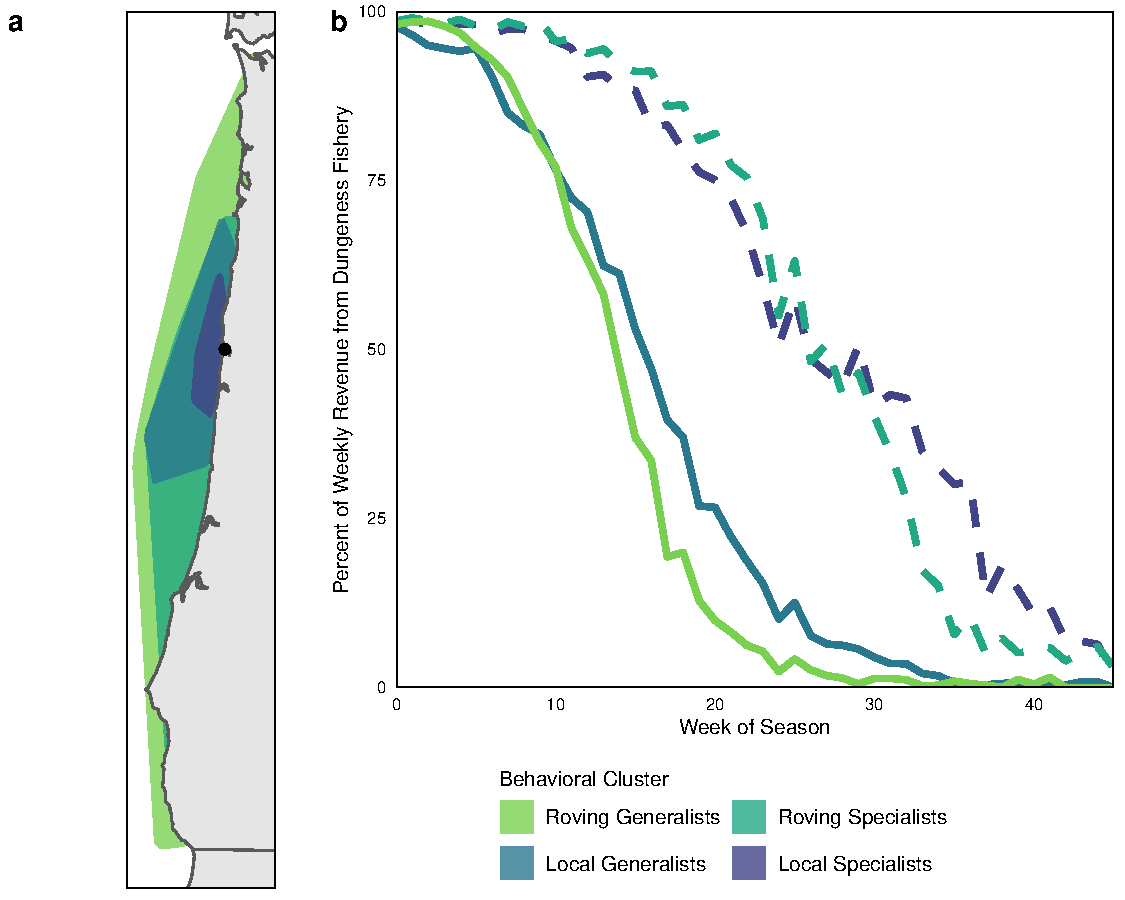
\includegraphics[width=\linewidth]{groups_mobility_flexibility.pdf}
\caption{Characteristic patterns in spatial mobility and fishery flexibility across behavioral groups in the west coast Dungeness crab fishery, exemplified by an Oregon port. (a) Fishing footprints of each behavioral group across all seasons for vessels originating from the Port of Newport, Oregon, USA. Shaded polygons are 95 percent convex hulls of all VMS locations for each group. (b) Fishery flexibility, displayed as the mean percent of total weekly revenue obtained from the Dungeness crab fishery (relative to all other fisheries) by vessels in each behavioral group. Weekly revenues are averaged across crab seasons and across all vessels in each group. Generalist groups are represented with solid lines, while Specialist groups are represented with dashed lines.}
\label{fig:characteristics}
\end{figure}

\hypertarget{behavioral-changes-during-the-marine-heatwave}{%
\subsection{Behavioral Changes During the Marine
Heatwave}\label{behavioral-changes-during-the-marine-heatwave}}

The four fishing behavioral groups defined by our cluster analysis
responded to the social-ecological disruption of the marine heatwave
(MHW) by increasing their dependence on other, non-Dungeness fisheries
and expanding their fishing ranges. All groups had higher non-Dungeness
fishery revenue during the MHW period than during other seasons,
indicating a potential fallback to other fisheries during a period of
delays and management disruptions in the crab fishery (Fig.
\ref{fig:revenue})(Fisher et al., 2021; Holland et al., 2020). The
2016-17 and 2017-18 seasons had the highest non-Dungeness crab revenue
in the time series (Fig. \ref{fig:revenue}a). The Generalist groups in
particular more than doubled their revenues from non-Dungeness fisheries
(ANOVA p \textless{} 0.01; Fig. \ref{fig:revenue}b). The Specialist
groups also had greater non-Dungeness revenues during the MHW period,
but the differences were not as substantial as for the Generalist groups
(Table S2, ANOVA p = 0.06 for Roving Specialists, p=0.99 for Local
Specialists).

Some Dungeness fishers also expanded their Dungeness crab fishing
grounds during the MHW, particularly the two Roving groups (Fig.
\ref{fig:homerange}). Prior to the MHW (2008-15), Roving Generalists had
the largest mean home range size at more than 4000 square kilometers
(Fig. \ref{fig:homerange}a). Roving Specialists had the second-largest
ranges on average (around 2500 square kilometers), while the Local
groups had much smaller ranges (less than 1000 square kilometers). In
the MHW period from 2015-18, the Roving groups fished significantly
larger areas, with the Roving Generalist and Roving Specialist groups
averaging more than 5500 and 3500 square kilometers fished, respectively
(p=0.001 and p\textless\textless0.001 for Roving Specialists and Roving
Generalists). In contrast, the areas fished for the Local groups did not
change significantly (Fig. \ref{fig:homerange}b and Table S3 ,
p\textgreater0.99 for both Local groups). For all four groups, within
the MHW period, the most pronounced change in mobility occurred during
the 2016-17 fishing season.

\begin{figure}%[tbhp]
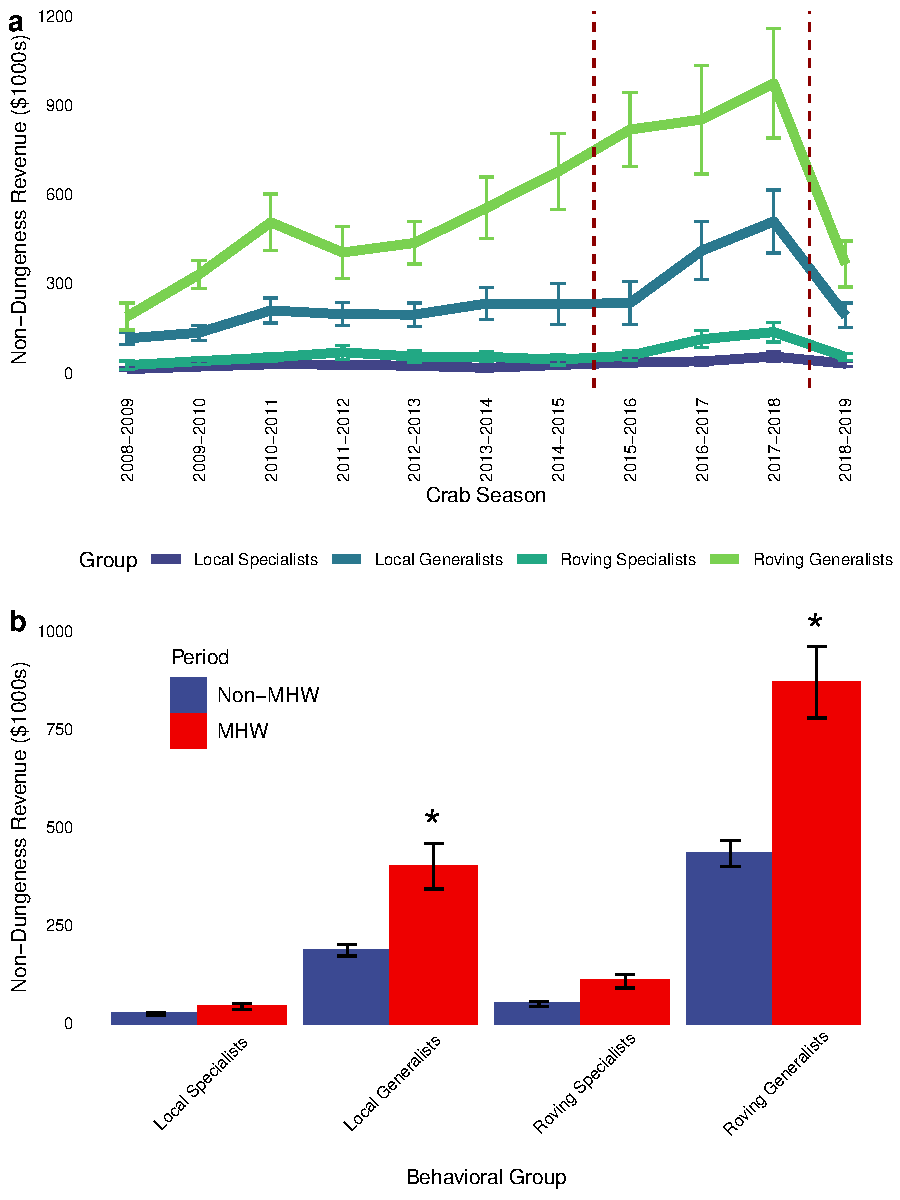
\includegraphics[width=\linewidth]{fig_nondcrb_revenue.pdf}
\caption{Non-Dungeness revenue for vessels in the analysis. (a) Seasonal mean revenue (+/- 2SE) for vessels in each behavioral group coming from all non-Dungeness fisheries combined. Vertical lines delineate the period of the marine heatwave (MHW). (b) Barplot of mean revenue (+/- 2SE) for vessels in each group during MHW and non-MHW seasons. Stars indicate groups with significantly different non-Dungeness revenue in MHW seasons.}
\label{fig:revenue}
\end{figure}

\hypertarget{profitability-of-behavioral-groups-during-the-marine-heatwave}{%
\subsection{Profitability of Behavioral Groups during the Marine
Heatwave}\label{profitability-of-behavioral-groups-during-the-marine-heatwave}}

An open question is whether the adaptive responses we detected and
quantified---greater spatial mobility and more flexible
fishing---allowed fishers to maintain profits in the face of this major
environmental perturbation. Our fishing cost model provides an
estimation of Dungeness crab profit (reported revenue minus estimated
cost) for every fishing trip in the data (i.e., for those vessels that
continued to fish), and allowed us to describe how profits within each
behavioral group varied over time (Fig. \ref{fig:profits}).

For all groups, average revenues and estimated costs both increased
during the MHW period (Figs. A.7, A.8), but revenue increases outweighed
the increases in cost, resulting in increased estimated profits.
Dungeness crab profits for all behavioral groups increased during the
MHW, significantly so for Local Generalists (p=0.05), Roving Generalists
(p\textless\textless.0001) and Roving Specialists (p=0.001, Table A.4).
The Roving Generalist group saw the largest increase in estimated
profits in both raw and percent increase in profits (more than a
\$63,000 increase per vessel, a 48 percent increase, on average). Local
Specialists experienced the smallest increase in profits of all groups
(25 percent) during the MHW, while Roving Specialists and Local
Generalists experienced a greater than 40 percent increase. In the
season after the dissipation of the MHW, estimated profits declined,
particularly for the Roving groups.

\hypertarget{discussion}{%
\section{Discussion}\label{discussion}}

The pace and magnitude of environmental change in the Anthropocene
demand assessment of how social-ecological systems will respond.
Ideally, management approaches can be designed to help humanity adapt by
meeting the basic needs of people without compromising ecosystems for
future generations (Lubchenco et al., 2016). As one of the last
remaining hunter--gatherer activities occurring at scale, commercial
fisheries offer an important lens through which to understand human
adaptations to novel and extreme conditions. The 2014-2016 marine
heatwave on the U.S. west coast stressed the adaptive ability of
participants in the highly lucrative Dungeness crab fishery, because an
environmental perturbation---the MHW and associated harmful algal bloom
and shoreward compression of large whale habitat---led to cascading
regulatory actions and market effects (Holland et al., 2020). Our
analysis revealed that Dungeness crab fishers that remained in the
fishery responded to unprecedented environmental and management changes
in multiple ways. Behavioral groups characterized by spatial mobility
used expanded fishing grounds in the 2016-17 and 2017-18 seasons to
maintain or increase revenues. Similarly, fishers with strategies based
around diversified fishing portfolios (Generalists) were able to
increase their revenue from other fisheries to bolster their total
fishing income. We found that vessels combining greater spatial mobility
with higher participation rates in other fisheries were the most
profitable, and that these financial benefits were maintained or
magnified during the MHW. The behavioral strategies observed in the
Dungeness crab fishery suggest that both portfolio and spatial
diversification pathways can improve adaptive capacity for human
harvesters across industrialized food systems during an era in which the
magnitude, frequency, and intensity of environmental perturbations are
increasing.

Our work builds on research from the economics (Gordon, 1954; Smith and
McKelvey, 1986), evolution (Gallagher et al., 2015), and ecology (Beever
et al., 2017) literatures investigating the relative ability of
specialists and generalists to cope with environmental change. The
cross-disciplinary consensus is that generalists may adapt better to
increasingly variable environments. Smith and McKelvey (1986) suggested
that specialists and generalists in fisheries use different strategies
to cope with variability and uncertainty in income---specialists are
efficient and minimize income risk through fishery-specific acumen,
while generalists hedge against risk by building diverse portfolios
(Kasperski and Holland, 2013; Oken et al., 2021). In a direct ecological
analogy, generalist consumers in an ecosystem experiencing novel
environmental conditions may be able to gain a competitive advantage
over specialists by efficiently switching to alternative prey sources
(Beever et al., 2017).

\begin{figure}%[tbhp]
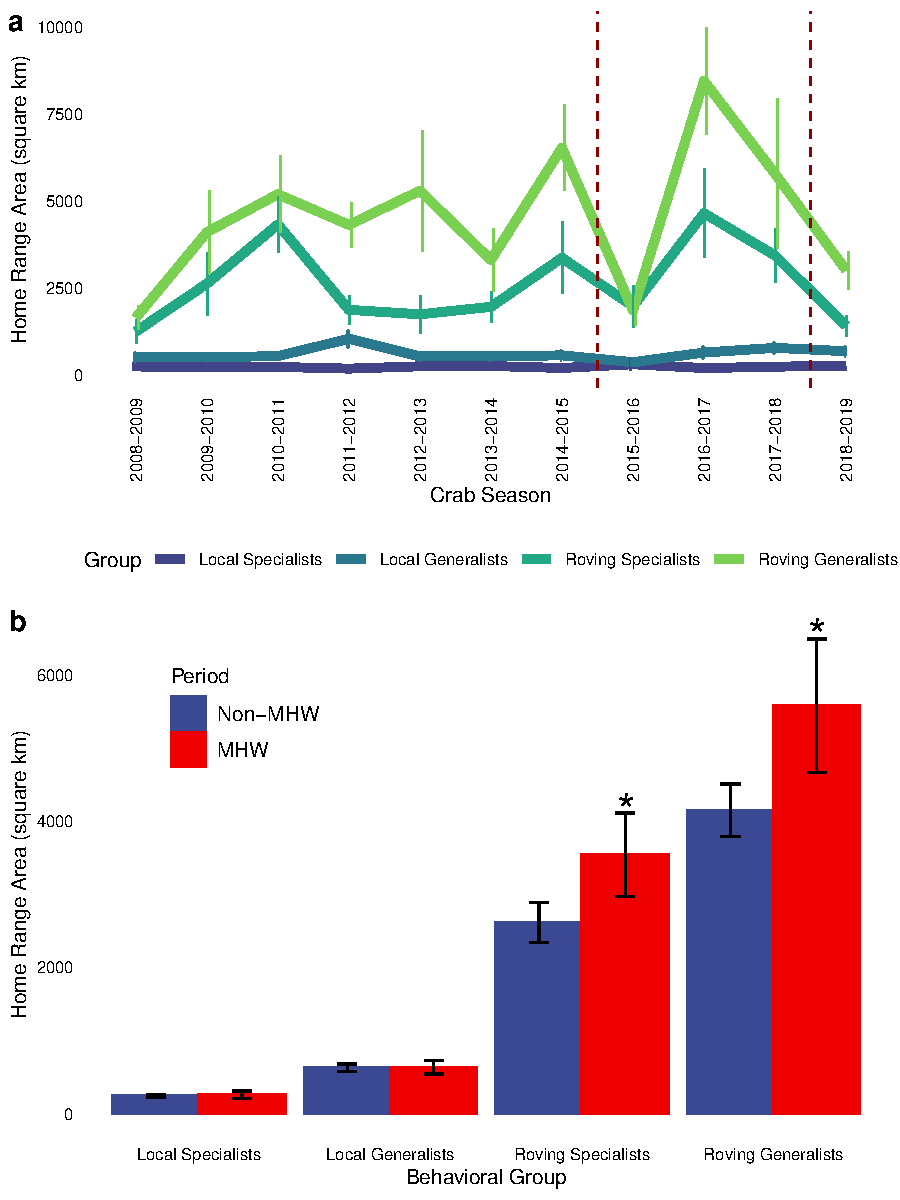
\includegraphics[width=\linewidth]{fig_homerange.pdf}
\caption{Home range (fishing area) size for vessels in the analysis. (a) Seasonal mean home range area in square kilometers (+/- 2SE) for vessels in each behavioral group. Vertical lines delineate the period of the MHW. (b) Barplot of mean home range area (+/- 2SE) for vessels in each group during MHW and non-MHW seasons. Stars indicate groups with significantly different home range size during MHW seasons.}
\label{fig:homerange}
\end{figure}

While management dynamics, markets, stochastic resource abundance, and
conditions in other fisheries are complicating factors (Holland et al.,
2020), the relative performance of specialist versus generalist
strategies in the Dungeness crab fishery largely adhere to these
existing economic and ecological models. Although some Specialists and
Generalists persisted through the MHW period, repeated environmental
disruptions in the future that cause further seasonal and spatial
restrictions on the Dungeness crab fishery may begin to favor a
Generalist, diversified strategy. Within the US west coast context,
existing fishery governance systems may constrain this type of
generalist adaptation (Kasperski and Holland, 2013; Russell et al.,
2018), but there are calls for ``climate-ready'' fisheries that include
the flexibility for fishers to move between fisheries (Wilson et al.,
2018). A better understanding of the social, economic, and cultural
drivers of fishers' decisions to be specialists or generalists is a core
component of a sustainable livelihoods approach to small-scale fisheries
management (Allison and Ellis, 2001; Finkbeiner, 2015). Such an approach
can also offer insights for the design of regulatory approaches that
facilitate resilience to environmental perturbation in larger-scale
fisheries and natural resource management contexts (Salas and Gaertner,
2004).

Diversification of fishery revenue was not the only axis of variation
associated with persistence in the face of the MHW. Spatial mobility was
also a key component of the fishing strategies we observed. Following
others who have used recently emerging technologies to understand the
sustainability of human harvester strategies (Brodie and Fragoso, 2020;
Frawley et al., 2020; Renner and Kuletz, 2015), we used satellite data
to characterize the spatial behavior of vessels. Roving groups, whether
Specialists or Generalists, were more profitable than their Local
counterparts under all conditions. The benefits of this spatial mobility
were clear during the marine heatwave. We hypothesize that Roving
vessels were the most capable of responding to management actions,
market forces, and ecological factors (e.g., product quantity and
quality) that shifted spatially during the heatwave. The ability of more
exploratory fishers to cope during an environmental disturbance has
recently been demonstrated in other commercial fisheries systems
(O'Farrell, Sanchirico, et al., 2019), and our findings confirm that
more mobile vessels performed better during the environmental
perturbation. Similar patterns have been shown among foraging marine
mammals, where individual animals that are more exploratory have greater
foraging success during anomalous climate conditions than more
site-faithful conspecifics (Abrahms et al., 2018).

Importantly, the nature of the data used in this study means that we
studied the behavior of the `survivors'---that is, the fishers who
decided or were able to remain in the Dungeness crab fishery during the
MHW period. The MHW acted as a selective force on Dungeness crab fishery
participation. Many Dungeness crab fishers during the 2016 and 2017
fishery closures chose (or were forced by circumstance) to not
participate in the fishery at all, instead opting to exit fishing
entirely or to re-concentrate all effort in alternative fisheries
(Fisher et al., 2021). Some of the relative success of the Dungeness
crab fishers during the MHW observed in this study, therefore, may be
due to reduced competition, as well as periods of supply shortages and
high prices. Although outside the scope of the current analysis, an
important area for further research is to determine how and why, when
faced with an environmental perturbation, fishers choose to remain or
exit a fishery (S. K. Moore et al., 2020).

With climate change expected to increase the frequency of extreme
environmental perturbations like MHWs (Oliver et al., 2018), established
patterns of natural resource management and human harvester behavior
will be challenged. In our study, following multiple adaptive pathways
by both diversifying and mobilizing appears to be one solution to an
extreme environmental event and rapid management changes in the
Dungeness crab fishery. Management measures that restrict the fishery
temporally or spatially---such as spatially-explicit biotoxin-related
closures or early termination of the fishing season due to risk of
interactions with protected or bycatch species---will differentially
affect distinct groups of fishers. Single-fishery specialists may thrive
when the harvested resource is stable and productive, but these fishers
may struggle to adapt if management measures restrict fishing season
lengths. Likewise, localized fishers can be successful through intimate
knowledge of fishing grounds, but if large-scale environmental
perturbations have spatially-explicit negative effects, fishers with
knowledge of a wider array of fishing grounds and greater mobility will
naturally gain an advantage (O'Farrell, Sanchirico, et al., 2019). Over
time, management context, or failures of management to adapt, can drive
changes in the makeup of fishing fleets as a whole (Frawley et al.,
2020). These changes are not inherently negative, but in order to
maintain the social, economic, and cultural benefits provided by a
fishery, managers should endeavour to anticipate behavioral changes
within fleets. More generally, these insights are congruent with an
evolving understanding of adaptation in complex social-ecological
systems (Lubchenco et al., 2016). Because complex systems are an
emergent product of the individual actions of human actors, informed
adaptive management requires an understanding of the drivers of
behaviors like those identified in this study along with well-calibrated
and nimble responses within governance systems.

\begin{figure}%[tbhp]
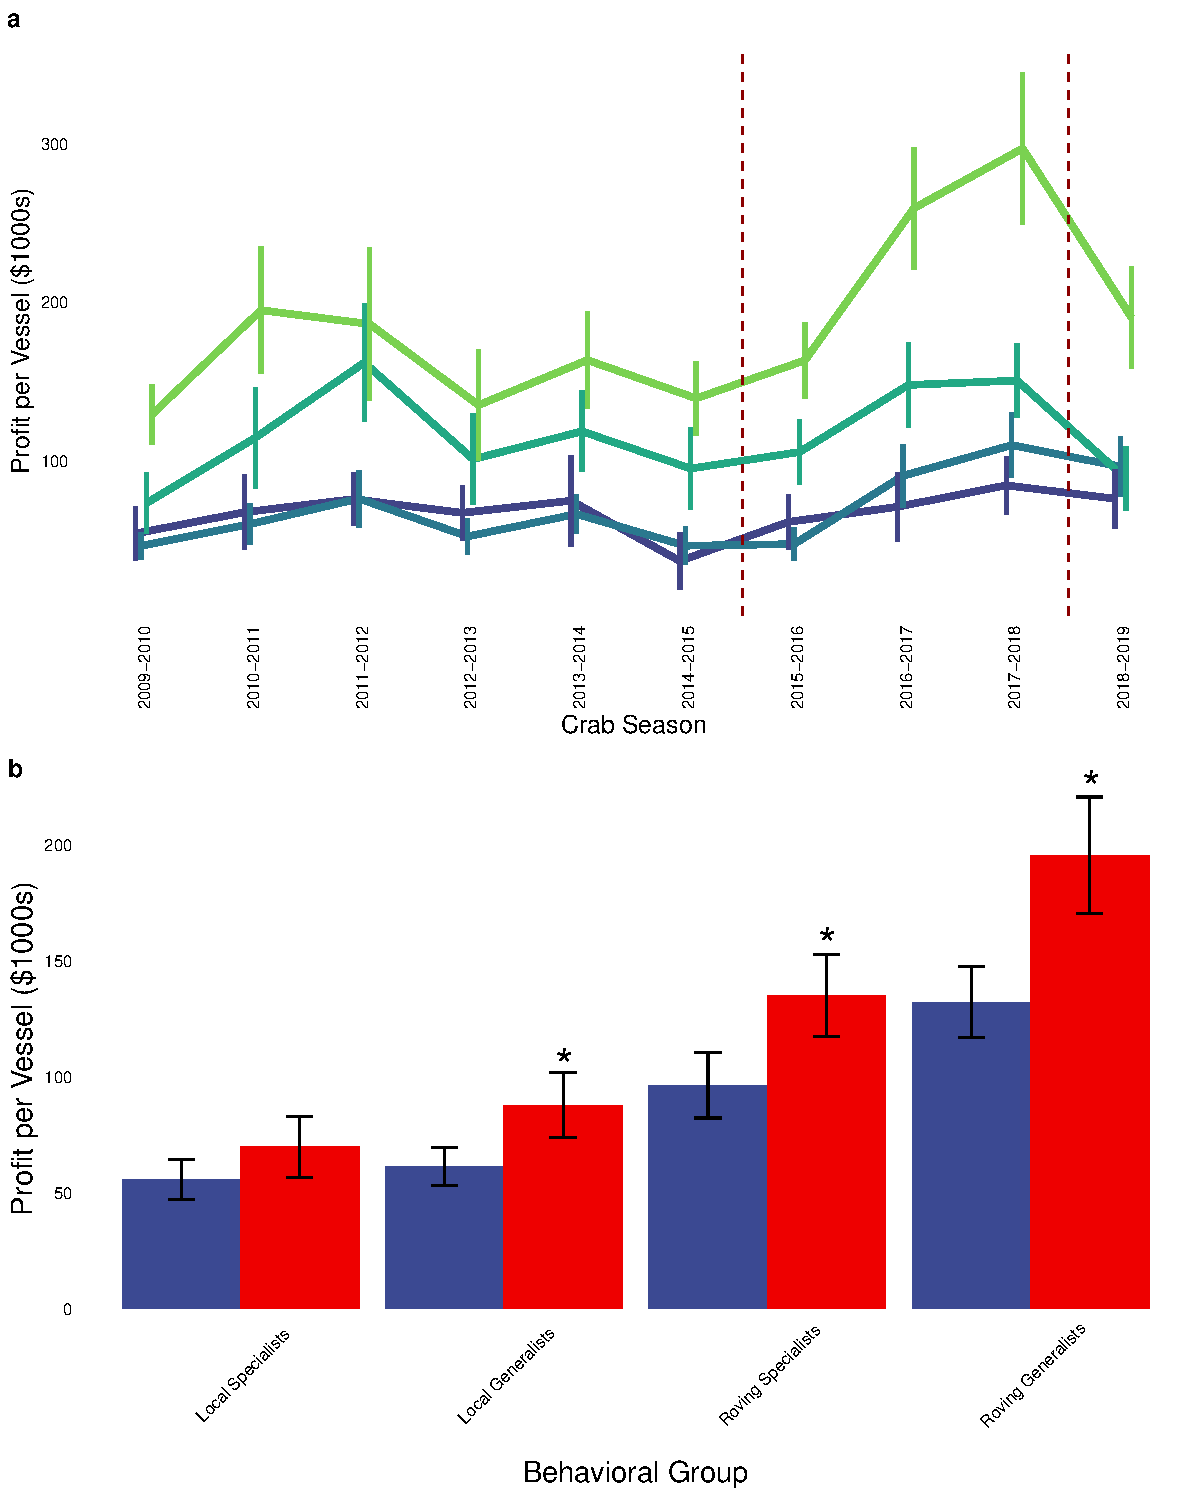
\includegraphics[width=\linewidth]{fig_profits.pdf}
\caption{Estimated profits by behavioral group. (a) Mean profit (+/- 2 SE) for vessels in each behavioral group over the full crab season. Vertical lines delineate the period of the marine heatwave. (b) Mean profit (+/- 2 SE) for each group in heatwave (MHW) versus non-MHW seasons. Stars indicate groups with significantly different estimated profits during MHW seasons.}
\label{fig:profits}
\end{figure}

For fishers and other human harvesters, future work using mixed methods
from the social sciences like participatory mapping and semi-structured
interviews (Frawley et al., 2020; S. K. Moore et al., 2020; Pellowe and
Leslie, 2019; Ritzman et al., 2018) will provide complementary insights
into the motivations and social drivers behind adaptive decisions, and
could help identify system-specific metrics of success or performance
beyond profitability. Furthermore, as integrated biophysical and
socioeconomic data streams become increasingly available for
environmental management (Bradley et al., 2019), data-driven,
interdisciplinary studies of resilience and adaptation will enable
dynamic management of natural resources (Hazen et al., 2018; Maxwell et
al., 2015). This push for the incorporation of multiple data streams in
environmental management extends beyond marine fisheries. For example,
in wildland fire management in the United States, integrated data
platforms that combine geospatial data with risk models and fuel
treatment scenarios are empowering adaptive fire management plans (Ager
et al., 2011; Krofcheck et al., 2018).

This study revealed the elements of behavioral diversity among human
harvesters in a lucrative, keystone commercial fishery, and described
how those elements enabled adaptation during an extreme environmental
event attributable to climate change (Hinder et al., 2012). Just as
biological response diversity can lead to enhanced ecosystem resilience
to environmental change (Elmqvist et al., 2003), behavioral diversity
among natural resource users may promote resilience of social-ecological
systems. Given the impending increase in extreme climatic events such as
marine heatwaves (Burge et al., 2014; Smale et al., 2019), recognition
of social and ecological traits that enable resilience now can help to
build toward a more prepared future. As quantitative data become
increasingly available in the United States and far beyond (Bradley et
al., 2019), behavioral analyses like ours can be used in the design of
adaptive management measures, to bolster policy analyses (Cabral et al.,
2018), and to inform decision-making under environmental uncertainty.

\hypertarget{refs}{%
\section*{References}\label{refs}}
\addcontentsline{toc}{section}{References}

\hypertarget{refs}{}
\leavevmode\hypertarget{ref-Abatzoglou2019}{}%
Abatzoglou, J.T., Williams, A.P., Barbero, R., 2019. Global emergence of
anthropogenic climate change in fire weather indices. Geophysical
Research Letters 46, 326--336.
doi:\href{https://doi.org/10.1029/2018GL080959}{10.1029/2018GL080959}

\leavevmode\hypertarget{ref-Abrahms2018}{}%
Abrahms, B., Hazen, E.L., Bograd, S.J., Brashares, J.S., Robinson, P.W.,
Scales, K.L., Crocker, D.E., Costa, D.P., 2018. Climate mediates the
success of migration strategies in a marine predator. Ecology Letters
21, 63--71.
doi:\href{https://doi.org/10.1111/ele.12871}{10.1111/ele.12871}

\leavevmode\hypertarget{ref-Ager2011}{}%
Ager, A.A., Vaillant, N.M., Finney, M.A., 2011. Integrating fire
behavior models and geospatial analysis for wildland fire risk
assessment and fuel management planning. Journal of Combustion 2011.
doi:\href{https://doi.org/10.1155/2011/572452}{10.1155/2011/572452}

\leavevmode\hypertarget{ref-Ellis2001}{}%
Allison, E.H., Ellis, F., 2001. The livelihoods approach and management
of small-scale fisheries. Marine Policy 25, 377--388.

\leavevmode\hypertarget{ref-Beever2017}{}%
Beever, E.A., Hall, L.E., Varner, J., Loosen, A.E., Dunham, J.B., Gahl,
M.K., Smith, F.A., Lawler, J.J., 2017. Behavioral flexibility as a
mechanism for coping with climate change. Frontiers in Ecology and the
Environment 15, 299--308.
doi:\href{https://doi.org/10.1002/fee.1502}{10.1002/fee.1502}

\leavevmode\hypertarget{ref-Bradley2019}{}%
Bradley, D., Merrifield, M., Miller, K.M., Lomonico, S., Wilson, J.R.,
Gleason, M.G., 2019. Opportunities to improve fisheries management
through innovative technology and advanced data systems. Fish and
Fisheries 20, 564--583.
doi:\href{https://doi.org/10.1111/faf.12361}{10.1111/faf.12361}

\leavevmode\hypertarget{ref-Branch2006}{}%
Branch, T.A., Hilborn, R., Haynie, A.C., Fay, G., Flynn, L., Griffiths,
J., Marshall, K.N., Randall, J.K., Scheuerell, J.M., Ward, E.J., Young,
M., 2006. Fleet dynamics and fishermen behavior: Lessons for fisheries
managers. Canadian Journal of Fisheries and Aquatic Sciences 63,
1647--1668.

\leavevmode\hypertarget{ref-Brodie2020}{}%
Brodie, J.F., Fragoso, J.M.V., 2020. Understanding the distribution of
bushmeat hunting effort across landscapes by testing hypotheses about
human foraging. Conservation Biology 0, 1--10.
doi:\href{https://doi.org/10.1111/cobi.13612}{10.1111/cobi.13612}

\leavevmode\hypertarget{ref-Burge2014}{}%
Burge, C.A., Eakin, C.M., Friedman, C.S., Froelich, B., Hershberger,
P.K., Hofmann, E.E., Petes, L.E., Prager, K.C., Weil, E., Willis, B.L.,
Ford, S.E., Harvell, C.D., 2014. Climate change influences on marine
infectious diseases: Implications for management and society. Annual
Review of Marine Science 6, 249--277.
doi:\href{https://doi.org/10.1146/annurev-marine-010213-135029}{10.1146/annurev-marine-010213-135029}

\leavevmode\hypertarget{ref-Cabral2018}{}%
Cabral, R.B., Mayorga, J., Clemence, M., Lynham, J., Koeshendrajana, S.,
Muawanah, U., Nugroho, D., Anna, Z., Ghofar, A., Zulbainarni, N.,
others, 2018. Rapid and lasting gains from solving illegal fishing.
Nature Ecology \& Evolution 2, 650--658.

\leavevmode\hypertarget{ref-Cavole2016}{}%
Cavole, L.M., Demko, A.M., Diner, R.E., Giddings, A., Koester, I.,
Pagniello, C.M., Paulsen, M.-L., Ramirez-Valdez, A., Schwenck, S.M.,
Yen, N.K., others, 2016. Biological impacts of the 2013--2015 warm-water
anomaly in the northeast pacific: Winners, losers, and the future.
Oceanography 29, 273--285.

\leavevmode\hypertarget{ref-nbclust2014}{}%
Charrad, M., Ghazzali, N., Boiteau, V., Niknafs, A., 2014. NbClust: An R
package for determining the relevant number of clusters in a data set.
Journal of Statistical Software 61, 1--36.

\leavevmode\hypertarget{ref-Cohen2007}{}%
Cohen, J.D., McClure, S.M., Yu, A.J., 2007. Should i stay or should i
go? How the human brain manages the trade-off between exploitation and
exploration. Philosophical Transactions of the Royal Society B:
Biological Sciences 362, 933--942.

\leavevmode\hypertarget{ref-Cook2018}{}%
Cook, B.I., Mankin, J.S., Anchukaitis, K.J., 2018. Climate change and
drought: From past to future. Current Climate Change Reports 4,
164--179.
doi:\href{https://doi.org/10.1007/s40641-018-0093-2}{10.1007/s40641-018-0093-2}

\leavevmode\hypertarget{ref-Dewees2004}{}%
Dewees, C.M., Sortais, K., Krachey, M.J., Hackett, S.C., Hankin, D.G.,
2004. Racing for crabs\ldots{} costs and management options evaluated in
dungeness crab fishery. California Agriculture 58, 186--189.
doi:\href{https://doi.org/10.3733/ca.v058n04p186}{10.3733/ca.v058n04p186}

\leavevmode\hypertarget{ref-Elmqvist2003a}{}%
Elmqvist, T., Folke, C., Nyström, M., Peterson, G., Bengtsson, J.,
Walker, B., Norberg, J., 2003. Response diversity, ecosystem change, and
resilience. Frontiers in Ecology and the Environment 1, 488--494.
doi:\href{https://doi.org/10.1890/1540-9295(2003)001\%5B0488:RDECAR\%5D2.0.CO;2}{10.1890/1540-9295(2003)001{[}0488:RDECAR{]}2.0.CO;2}

\leavevmode\hypertarget{ref-Feist2021}{}%
Feist, B.E., Samhouri, J.F., Forney, K.A., Saez, L.E., 2021. Footprints
of fixed-gear fisheries in relation to rising whale entanglements on the
u.s. West coast. Fisheries Management and Ecology 28, 283--294.
doi:\href{https://doi.org/10.1111/fme.12478}{10.1111/fme.12478}

\leavevmode\hypertarget{ref-Finkbeiner2015}{}%
Finkbeiner, E.M., 2015. The role of diversification in dynamic
small-scale fisheries: Lessons from baja california sur, mexico. Global
Environmental Change 32, 139--152.
doi:\href{https://doi.org/10.1016/j.gloenvcha.2015.03.009}{10.1016/j.gloenvcha.2015.03.009}

\leavevmode\hypertarget{ref-Fisher2021}{}%
Fisher, M.C., Moore, S.K., Jardine, S.L., Watson, J.R., Samhouri, J.F.,
2021. Climate shock effects and mediation in fisheries. Proceedings of
the National Academy of Sciences of the United States of America 118,
1--8.
doi:\href{https://doi.org/10.1073/pnas.2014379117}{10.1073/pnas.2014379117}

\leavevmode\hypertarget{ref-Frawley2020}{}%
Frawley, T.H., Muhling, B.A., Brodie, S., Fisher, M.C., Tommasi, D.,
Fol, G.L., Hazen, E.L., Stohs, S.S., Finkbeiner, E.M., Jacox, M.G.,
2020. Changes to the structure and function of an albacore fishery
reveal shifting social-ecological realities for pacific northwest
fishermen 1--18.
doi:\href{https://doi.org/10.1111/faf.12519}{10.1111/faf.12519}

\leavevmode\hypertarget{ref-Fryxell2017}{}%
Fryxell, J.M., Hilborn, R., Bieg, C., Turgeon, K., Caskenette, A.,
McCann, K.S., 2017. Supply and demand drive a critical transition to
dysfunctional fisheries. Proceedings of the National Academy of Sciences
of the United States of America 114, 12333--12337.
doi:\href{https://doi.org/10.1073/pnas.1705525114}{10.1073/pnas.1705525114}

\leavevmode\hypertarget{ref-Fuller2017}{}%
Fuller, E.C., Samhouri, J.F., Stoll, J.S., Levin, S.A., Watson, J.R.,
2017. Characterizing fisheries connectivity in marine social-ecological
systems. ICES Journal of Marine Science 74, 2087--2096.
doi:\href{https://doi.org/10.1093/icesjms/fsx128}{10.1093/icesjms/fsx128}

\leavevmode\hypertarget{ref-Fulton2011h}{}%
Fulton, E.A., Smith, A.D.M., Smith, D.C., Putten, I.E.V., 2011. Human
behaviour: The key source of uncertainty in fisheries management. Fish
and Fisheries 12, 2--17.
doi:\href{https://doi.org/10.1111/j.1467-2979.2010.00371.x}{10.1111/j.1467-2979.2010.00371.x}

\leavevmode\hypertarget{ref-Gallagher2015}{}%
Gallagher, A.J., Hammerschlag, N., Cooke, S.J., Costa, D.P., Irschick,
D.J., 2015. Evolutionary theory as a tool for predicting extinction
risk. Trends in Ecology and Evolution 30, 61--65.
doi:\href{https://doi.org/10.1016/j.tree.2014.12.001}{10.1016/j.tree.2014.12.001}

\leavevmode\hypertarget{ref-Gladics2017}{}%
Gladics, A.J., Melvin, E.F., Suryan, R.M., Good, T.P., Jannot, J.E.,
Guy, T.J., 2017. Fishery-specific solutions to seabird bycatch in the
u.s. West coast sablefish fishery. Fisheries Research 196, 85--95.
doi:\href{https://doi.org/10.1016/j.fishres.2017.08.015}{10.1016/j.fishres.2017.08.015}

\leavevmode\hypertarget{ref-Gordon1954}{}%
Gordon, H.S., 1954. The economic theory of a common-property resource:
The fishery. The Journal of Political Economy 124--142.

\leavevmode\hypertarget{ref-Hamilton2019}{}%
Hamilton, S., Baker, G.B., 2019. Technical mitigation to reduce marine
mammal bycatch and entanglement in commercial fishing gear: Lessons
learnt and future directions. Reviews in Fish Biology and Fisheries 29,
223--247.
doi:\href{https://doi.org/10.1007/s11160-019-09550-6}{10.1007/s11160-019-09550-6}

\leavevmode\hypertarget{ref-Kohin2018}{}%
Hazen, E.L., Scales, K.L., Maxwell, S.M., Briscoe, D.K., Welch, H.,
Bograd, S.J., Bailey, H., Benson, S.R., Eguchi, T., Dewar, H., Kohin,
S., Costa, D.P., Crowder, L.B., Lewison, R.L., 2018. A dynamic ocean
management tool to reduce bycatch and support sustainable fisheries.
Science Advances 4, eaar3001.
doi:\href{https://doi.org/10.1126/sciadv.aar3001}{10.1126/sciadv.aar3001}

\leavevmode\hypertarget{ref-Hilborn1985}{}%
Hilborn, R., 1985. Fleet dynamics and individual variation: Why some
people catch more fish than others. Canadian Journal of Fisheries and
Aquatic Sciences 42, 2--13.
doi:\href{https://doi.org/10.1139/f85-001}{10.1139/f85-001}

\leavevmode\hypertarget{ref-Hinder2012}{}%
Hinder, S.L., Hays, G.C., Edwards, M., Roberts, E.C., Walne, A.W.,
Gravenor, M.B., 2012. Changes in marine dinoflagellate and diatom
abundance under climate change. Nature Climate Change 2, 271--275.
doi:\href{https://doi.org/10.1038/nclimate1388}{10.1038/nclimate1388}

\leavevmode\hypertarget{ref-Holland2020}{}%
Holland, D.S., Abbott, J.K., Norman, K.E., 2020. Fishing to live or
living to fish: Job satisfaction and identity of west coast fishermen.
Ambio 49, 628--639.
doi:\href{https://doi.org/10.1007/s13280-019-01206-w}{10.1007/s13280-019-01206-w}

\leavevmode\hypertarget{ref-Holland2020a}{}%
Holland, D.S., Leonard, J., 2020. Is a delay a disaster? Economic
impacts of the delay of the california dungeness crab fishery due to a
harmful algal bloom. Harmful Algae 98, 101904.
doi:\href{https://doi.org/10.1016/j.hal.2020.101904}{10.1016/j.hal.2020.101904}

\leavevmode\hypertarget{ref-Holland2017}{}%
Holland, D.S., Speir, C., Agar, J., Crosson, S., Depiper, G., Kasperski,
S., Kitts, A.W., Perruso, L., 2017. Impact of catch shares on
diversification of fishers' income and risk. Proceedings of the National
Academy of Sciences of the United States of America 114, 9302--9307.
doi:\href{https://doi.org/10.1073/pnas.1702382114}{10.1073/pnas.1702382114}

\leavevmode\hypertarget{ref-Jardine2020}{}%
Jardine, S.L., Fisher, M.C., Moore, S.K., Samhouri, J.F., 2020.
Inequality in the economic impacts from climate shocks in fisheries: The
case of harmful algal blooms. Ecological Economics 176, 106691.
doi:\href{https://doi.org/10.1016/j.ecolecon.2020.106691}{10.1016/j.ecolecon.2020.106691}

\leavevmode\hypertarget{ref-Joo2015}{}%
Joo, R., Salcedo, O., Gutierrez, M., Fablet, R., Bertrand, S., 2015.
Defining fishing spatial strategies from vms data: Insights from the
world's largest monospecific fishery. Fisheries Research 164, 223--230.
doi:\href{https://doi.org/10.1016/j.fishres.2014.12.004}{10.1016/j.fishres.2014.12.004}

\leavevmode\hypertarget{ref-Kasperski2013}{}%
Kasperski, S., Holland, D.S., 2013. Income diversification and risk for
fishermen. Proceedings of the National Academy of Sciences 110,
2076--2081.

\leavevmode\hypertarget{ref-Krofcheck2018}{}%
Krofcheck, D.J., Hurteau, M.D., Scheller, R.M., Loudermilk, E.L., 2018.
Prioritizing forest fuels treatments based on the probability of
high-severity fire restores adaptive capacity in sierran forests. Global
Change Biology 24, 729--737.
doi:\href{https://doi.org/10.1111/gcb.13913}{10.1111/gcb.13913}

\leavevmode\hypertarget{ref-Leslie2015}{}%
Leslie, H.M., Basurto, X., Nenadovic, M., Sievanen, L., Cavanaugh, K.C.,
Cota-Nieto, J.J., Erisman, B.E., Finkbeiner, E., Hinojosa-Arango, G.,
Moreno-Báez, M., Nagavarapu, S., Reddy, S.M.W., Sánchez-Rodríguez, A.,
Siegel, K., Ulibarria-Valenzuela, J.J., Weaver, A.H., Aburto-Oropeza,
O., 2015. Operationalizing the social-ecological systems framework to
assess sustainability. Proceedings of the National Academy of Sciences
of the United States of America 112, 5979--5984.
doi:\href{https://doi.org/10.1073/pnas.1414640112}{10.1073/pnas.1414640112}

\leavevmode\hypertarget{ref-Wiener2003}{}%
Liaw, A., Wiener, M., 2002. Classification and regression by
randomForest. R News 3, 18--22.

\leavevmode\hypertarget{ref-VanLoon2016}{}%
Loon, A.F.V., Gleeson, T., Clark, J., Dijk, A.I.J.V., Stahl, K.,
Hannaford, J., Baldassarre, G.D., Teuling, A.J., Tallaksen, L.M.,
Uijlenhoet, R., Hannah, D.M., Sheffield, J., Svoboda, M., Verbeiren, B.,
Wagener, T., Rangecroft, S., Wanders, N., Lanen, H.A.J.V., 2016. Drought
in the anthropocene. Nature Geoscience 9, 89--91.
doi:\href{https://doi.org/10.1038/ngeo2646}{10.1038/ngeo2646}

\leavevmode\hypertarget{ref-Lubchenco2016}{}%
Lubchenco, J., Cerny-Chipman, E.B., Reimer, J.N., Levin, S.A., 2016. The
right incentives enable ocean sustainability successes and provide hope
for the future. Proceedings of the National Academy of Sciences of the
United States of America 113, 14507--14514.
doi:\href{https://doi.org/10.1073/pnas.1604982113}{10.1073/pnas.1604982113}

\leavevmode\hypertarget{ref-Mao2020}{}%
Mao, J., Jardine, S.L., 2020. Market impacts of a toxic algae event: The
case of california dungeness crab. Marine Resource Economics 35, 1--20.
doi:\href{https://doi.org/10.1086/707643}{10.1086/707643}

\leavevmode\hypertarget{ref-Maxwell2015}{}%
Maxwell, S.M., Hazen, E.L., Lewison, R.L., Dunn, D.C., Bailey, H.,
Bograd, S.J., Briscoe, D.K., Fossette, S., Hobday, A.J., Bennett, M.,
Benson, S., Caldwell, M.R., Costa, D.P., Dewar, H., Eguchi, T., Hazen,
L., Kohin, S., Sippel, T., Crowder, L.B., 2015. Dynamic ocean
management: Defining and conceptualizing real-time management of the
ocean. Marine Policy 58, 42--50.
doi:\href{https://doi.org/10.1016/j.marpol.2015.03.014}{10.1016/j.marpol.2015.03.014}

\leavevmode\hypertarget{ref-McCabe2016a}{}%
McCabe, R.M., Hickey, B.M., Kudela, R.M., Lefebvre, K.A., Adams, N.G.,
Bill, B.D., Gulland, F.M.D., Thomson, R.E., Cochlan, W.P., Trainer,
V.L., 2016. An unprecedented coastwide toxic algal bloom linked to
anomalous ocean conditions. Geophysical Research Letters 43, 10,
366--10, 376.
doi:\href{https://doi.org/10.1002/2016GL070023}{10.1002/2016GL070023}

\leavevmode\hypertarget{ref-Mcginnis2014}{}%
Mcginnis, M.D., Ostrom, E., 2014. Social-ecological system framework :
Initial changes and continuing challenges. Ecology and Society 19.

\leavevmode\hypertarget{ref-Mendo2019}{}%
Mendo, T., Smout, S., Photopoulou, T., James, M., 2019. Identifying
fishing grounds from vessel tracks: Model-based inference for small
scale fisheries. Royal Society Open Science 6.
doi:\href{https://doi.org/10.1098/rsos.191161}{10.1098/rsos.191161}

\leavevmode\hypertarget{ref-Moore2020harmful}{}%
Moore, K.M., Allison, E.H., Dreyer, S.J., Ekstrom, J.A., Jardine, S.L.,
Klinger, T., Moore, S.K., Norman, K.C., 2020. Harmful algal blooms:
Identifying effective adaptive actions used in fishery-dependent
communities in response to a protracted event. Frontiers in Marine
Science 6, 803.

\leavevmode\hypertarget{ref-Moore2020}{}%
Moore, S.K., Dreyer, S.J., Ekstrom, J.A., Moore, K., Norman, K.,
Klinger, T., Allison, E.H., Jardine, S.L., 2020. Harmful algal blooms
and coastal communities: Socioeconomic impacts and actions taken to cope
with the 2015 u.s. West coast domoic acid event. Harmful Algae 96,
101799.
doi:\href{https://doi.org/10.1016/j.hal.2020.101799}{10.1016/j.hal.2020.101799}

\leavevmode\hypertarget{ref-OFarrell2019}{}%
O'Farrell, S., Chollett, I., Sanchirico, J.N., Perruso, L., 2019.
Classifying fishing behavioral diversity using high-frequency movement
data. Proceedings of the National Academy of Sciences 116, 16811--16816.
doi:\href{https://doi.org/10.1073/pnas.1906766116}{10.1073/pnas.1906766116}

\leavevmode\hypertarget{ref-OFarrell2019a}{}%
O'Farrell, S., Sanchirico, J.N., Spiegel, O., Depalle, M., Haynie, A.C.,
Murawski, S.A., Perruso, L., Strelcheck, A., 2019. Disturbance modifies
payoffs in the explore-exploit trade-off. Nature Communications 10,
1--9.
doi:\href{https://doi.org/10.1038/s41467-019-11106-y}{10.1038/s41467-019-11106-y}

\leavevmode\hypertarget{ref-Oken2021}{}%
Oken, K.L., Holland, D.S., Andr´, A., Punt, A.E., 2021. The effects of
population synchrony, life history, and access constraints on benefits
from fishing portfolios.

\leavevmode\hypertarget{ref-Oliver2018}{}%
Oliver, E.C.J., Donat, M.G., Burrows, M.T., Moore, P.J., Smale, D.A.,
Alexander, L.V., Benthuysen, J.A., Feng, M., Gupta, A.S., Hobday, A.J.,
Holbrook, N.J., Perkins-Kirkpatrick, S.E., Scannell, H.A., Straub, S.C.,
Wernberg, T., 2018. Longer and more frequent marine heatwaves over the
past century. Nature Communications 9, 1--12.
doi:\href{https://doi.org/10.1038/s41467-018-03732-9}{10.1038/s41467-018-03732-9}

\leavevmode\hypertarget{ref-Pellowe2019}{}%
Pellowe, K.E., Leslie, H.M., 2019. Heterogeneity among clam harvesters
in northwest mexico shapes individual adaptive capacity. Ecology and
Society 24.
doi:\href{https://doi.org/10.5751/ES-11297-240425}{10.5751/ES-11297-240425}

\leavevmode\hypertarget{ref-Pfeiffer2016}{}%
Pfeiffer, L., Gratz, T., 2016. The effect of rights-based fisheries
management on risk taking and fishing safety. Proceedings of the
National Academy of Sciences of the United States of America 113,
2615--2620.
doi:\href{https://doi.org/10.1073/pnas.1509456113}{10.1073/pnas.1509456113}

\leavevmode\hypertarget{ref-Rasmuson2013}{}%
Rasmuson, L.K., 2013. The biology, ecology and fishery of the dungeness
crab, cancer magister, 1st ed, Advances in Marine Biology. Elsevier Ltd.
doi:\href{https://doi.org/10.1016/B978-0-12-410498-3.00003-3}{10.1016/B978-0-12-410498-3.00003-3}

\leavevmode\hypertarget{ref-RCoreTeam2021}{}%
R Core Team, 2021. R: A language and environment for statistical
computing. R Foundation for Statistical Computing, Vienna, Austria.

\leavevmode\hypertarget{ref-Renner2015}{}%
Renner, M., Kuletz, K.J., 2015. A spatial-seasonal analysis of the
oiling risk from shipping traffic to seabirds in the aleutian
archipelago. Marine Pollution Bulletin 101, 127--136.
doi:\href{https://doi.org/10.1016/j.marpolbul.2015.11.007}{10.1016/j.marpolbul.2015.11.007}

\leavevmode\hypertarget{ref-Richerson2020}{}%
Richerson, K., Punt, A.E., Holland, D.S., 2020. Nearly a half century of
high but sustainable exploitation in the dungeness crab (cancer
magister) fishery. Fisheries Research 226, 105528.
doi:\href{https://doi.org/10.1016/j.fishres.2020.105528}{10.1016/j.fishres.2020.105528}

\leavevmode\hypertarget{ref-Ritzman2018}{}%
Ritzman, J., Brodbeck, A., Brostrom, S., McGrew, S., Dreyer, S.,
Klinger, T., Moore, S.K., 2018. Economic and sociocultural impacts of
fisheries closures in two fishing-dependent communities following the
massive 2015 u.s. West coast harmful algal bloom. Harmful Algae 80,
35--45.
doi:\href{https://doi.org/10.1016/j.hal.2018.09.002}{10.1016/j.hal.2018.09.002}

\leavevmode\hypertarget{ref-Russell2018}{}%
Russell, S.M., Oostenburg, M.V., Vizek, A., 2018. Adapting to catch
shares: Perspectives of west coast groundfish trawl participants.
Coastal Management 46, 603--620.
doi:\href{https://doi.org/10.1080/08920753.2018.1522491}{10.1080/08920753.2018.1522491}

\leavevmode\hypertarget{ref-Salas2004a}{}%
Salas, S., Gaertner, D., 2004. The behavioural dynamics of fishers:
Management implications. Fish and Fisheries 5, 153--167.
doi:\href{https://doi.org/10.1111/j.1467-2979.2004.00146.x}{10.1111/j.1467-2979.2004.00146.x}

\leavevmode\hypertarget{ref-Santora2020}{}%
Santora, J.A., Mantua, N.J., Schroeder, I.D., Field, J.C., Hazen, E.L.,
Bograd, S.J., Sydeman, W.J., Wells, B.K., Calambokidis, J., Saez, L.,
Lawson, D., Forney, K.A., 2020. Habitat compression and ecosystem shifts
as potential links between marine heatwave and record whale
entanglements. Nature Communications 2020 11:1 11, 1--12.
doi:\href{https://doi.org/10.1038/s41467-019-14215-w}{10.1038/s41467-019-14215-w}

\leavevmode\hypertarget{ref-Smale2019}{}%
Smale, D.A., Wernberg, T., Oliver, E.C.J., Thomsen, M., Harvey, B.P.,
Straub, S.C., Burrows, M.T., Alexander, L.V., Benthuysen, J.A., Donat,
M.G., Feng, M., Hobday, A.J., Holbrook, N.J., Perkins-Kirkpatrick, S.E.,
Scannell, H.A., Gupta, A.S., Payne, B.L., Moore, P.J., 2019. Marine
heatwaves threaten global biodiversity and the provision of ecosystem
services. Nature Climate Change 9, 306--312.
doi:\href{https://doi.org/10.1038/s41558-019-0412-1}{10.1038/s41558-019-0412-1}

\leavevmode\hypertarget{ref-Smith1986}{}%
Smith, C.L., McKelvey, R., 1986. Specialist and generalist: Roles for
coping with variability. North American Journal of Fisheries Management
6, 88--99.
doi:\href{https://doi.org/10.1577/1548-8659(1986)6\%3C88:sag\%3E2.0.co;2}{10.1577/1548-8659(1986)6\textless88:sag\textgreater2.0.co;2}

\leavevmode\hypertarget{ref-Suryan2021}{}%
Suryan, R.M., Arimitsu, M.L., Coletti, H.A., Hopcroft, R.R., Lindeberg,
M.R., Barbeaux, S.J., Batten, S.D., Burt, W.J., Bishop, M.A., Bodkin,
J.L., Brenner, R., Campbell, R.W., Cushing, D.A., Danielson, S.L., Dorn,
M.W., Drummond, B., Esler, D., Gelatt, T., Hanselman, D.H., Hatch, S.A.,
Haught, S., Holderied, K., Iken, K., Irons, D.B., Kettle, A.B., Kimmel,
D.G., Konar, B., Kuletz, K.J., Laurel, B.J., Maniscalco, J.M., Matkin,
C., McKinstry, C.A.E., Monson, D.H., Moran, J.R., Olsen, D., Palsson,
W.A., Pegau, W.S., Piatt, J.F., Rogers, L.A., Rojek, N.A., Schaefer, A.,
Spies, I.B., Straley, J.M., Strom, S.L., Sweeney, K.L., Szymkowiak, M.,
Weitzman, B.P., Yasumiishi, E.M., Zador, S.G., 2021. Ecosystem response
persists after a prolonged marine heatwave. Scientific Reports 11,
1--17.
doi:\href{https://doi.org/10.1038/s41598-021-83818-5}{10.1038/s41598-021-83818-5}

\leavevmode\hypertarget{ref-Townhill2018}{}%
Townhill, B.L., Tinker, J., Jones, M., Pitois, S., Creach, V., Simpson,
S.D., Dye, S., Bear, E., Pinnegar, J.K., 2018. Harmful algal blooms and
climate change: Exploring future distribution changes. ICES Journal of
Marine Science 75, 1882--1893.
doi:\href{https://doi.org/10.1093/icesjms/fsy113}{10.1093/icesjms/fsy113}

\leavevmode\hypertarget{ref-VonBiela2019}{}%
von Biela, V., Arimitsu, M.L., Piatt, J.F., Heflin, B.M., Schoen, S.,
2019. Extreme reduction in condition of a key forage fish during the
pacific marine heatwave of 2014--2016. Marine Ecology Progress Series
613, 171--182.

\leavevmode\hypertarget{ref-Watson2016a}{}%
Watson, J.T., Haynie, A.C., 2016. Using vessel monitoring system data to
identify and characterize trips made by fishing vessels in the united
states north pacific. PLoS ONE 11, 1--20.
doi:\href{https://doi.org/10.1371/journal.pone.0165173}{10.1371/journal.pone.0165173}

\leavevmode\hypertarget{ref-Wilson2018}{}%
Wilson, J.R., Lomonico, S., Bradley, D., Sievanen, L., Dempsey, T.,
Bell, M., McAfee, S., Costello, C., Szuwalski, C., McGonigal, H.,
Fitzgerald, S., Gleason, M., 2018. Adaptive comanagement to achieve
climate-ready fisheries. Conservation Letters 11, 1--7.
doi:\href{https://doi.org/10.1111/conl.12452}{10.1111/conl.12452}

\leavevmode\hypertarget{ref-Young2019}{}%
Young, T., Fuller, E.C., Provost, M.M., Coleman, K.E., Martin, K.S.,
McCay, B.J., Pinsky, M.L., 2019. Adaptation strategies of coastal
fishing communities as species shift poleward. ICES Journal of Marine
Science 76, 93--103.
doi:\href{https://doi.org/10.1093/icesjms/fsy140}{10.1093/icesjms/fsy140}


\end{document}

